\chapter{Data structures for Fortune's algorithm}

During the algorithm we will need three data structures:
\begin{itemize}
    \item A \textbf{priority queue} $\mathcal{Q}$ for keeping track of the site and circle events.
    \item A \textbf{doubly-connected edge list (DCEL)} $\mathcal{D}$ for keeping track of the current state of the Voronoi diagram. See Definition \ref{defn:dcel}. This will be updated after each site and circle event.
    \item A self-balancing \textbf{binary search tree (BST)} $\mathcal{T}$ for keeping track of the breakpoints and arcs on the beach line.
\end{itemize}
We explain them in detail in the next sections.

\section{Priority queue}
The priority queue stores the site and circle events, and enables the algorithm to handle them in order. Each element in the priority queue has a priority. For a site event the $y$-value of the point describes the priority, and for a circle event the priority is given by the $y$-value of the lowest point of the center of the circle which describes the event. Site events also store a pointer to the site, and circle events also store the center of its definining circle and a pointer to the arc in $\mathcal{T}$ which is disappearing.

For the implementation of the priority queue we will use a binary heap. These are described in CLRS \todo{Ref}, and the implementation has been taken from \todo{Ref}.

\section{Binary search tree}
We will store the current configuration of the beach line in a binary search tree, which has some additional information stored:
\begin{itemize}
    \item Leaves correspond to arcs on the beach line. Every leaf has a pointer to a site in $P$, and it also has a pointer to a potential circle event at which the arc will disappear. If no circle event has been detected yet, the pointer will simply be \textsc{nil}. Every arc will also store \textsf{.leftArc} and \textsf{.rightArc} pointers to the two arcs that surround it, so that we get a doubly linked list of arcs that are currently on the beach line. These pointers are \textsc{nil} if the leaf has no neighbour in that particular direction. In our figures the leaves will be depicted by squares.
    
    \item Internal nodes correspond to breakpoints on the beach line. Every breakpoint stores an ordered pair $(p, q)$, where $p$ and $q$ are sites in $P$. The order is important since the intersection of the hyperbolas defined by $p$ and $q$ consists of two points, and the order lets us tell these breakpoints apart. If we consider the beach line as running from the left to the right, then at every breakpoint an arc is leaving, and another is entering it. Thus the tuple $(p, q)$ tells us that we are interested in the breakpoint at which an arc pointing to $p$ leaves, and an arc pointing to $q$ is entering. In our figures the internal nodes will be depicted by circles.
\end{itemize}

The binary tree will only be updated at site and circle events. First we describe what happens at a site event.

During the first site event, the tree will be empty (we say it is \textsc{nil}), so to add an arc $\alpha$ to it, we simply turn the tree into a leaf, which describes the new arc, and we have it point to the first site $p$, illustrated as follows:
\[
    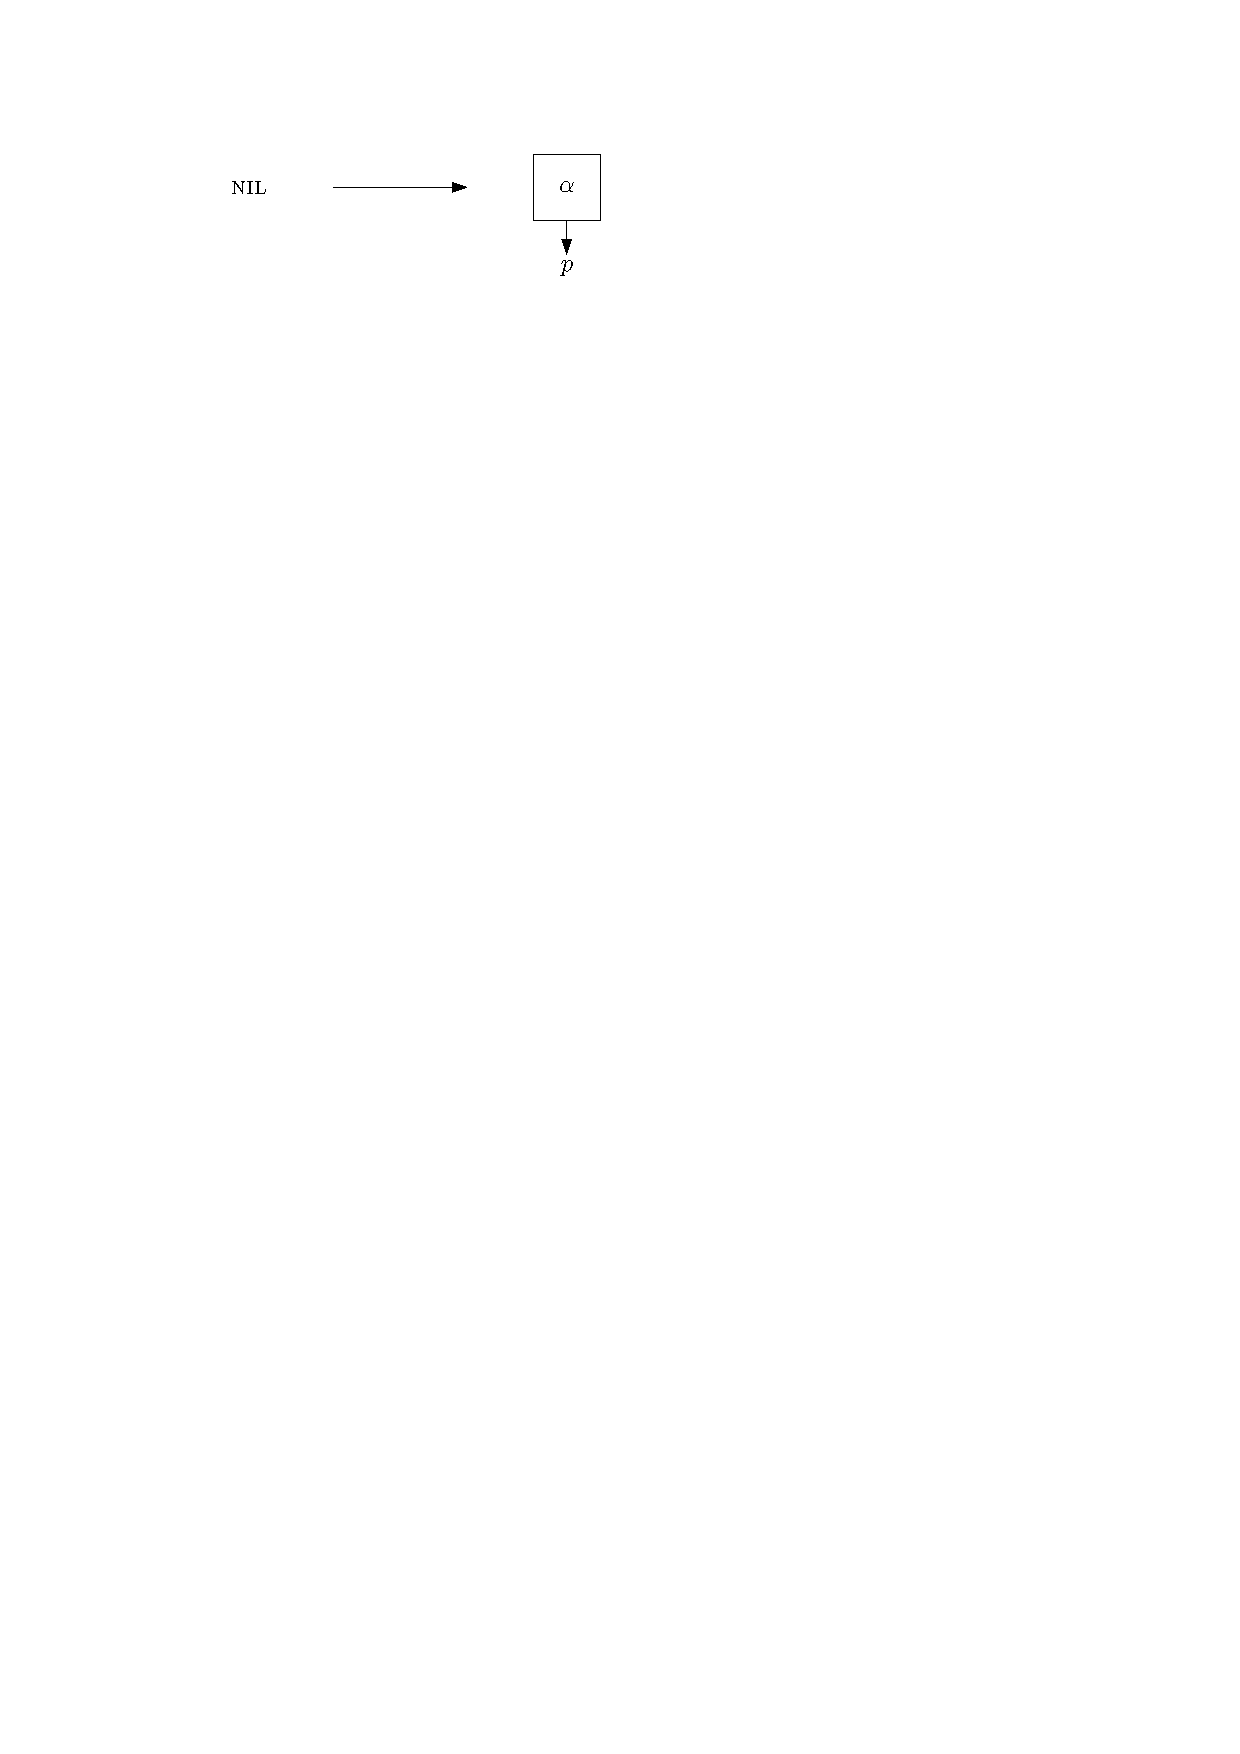
\includegraphics[scale=0.75]{images/tree_insert_base}
\]
Now we look at the general case. We assume that $\alpha$ is an arc on the beach line, which points to a point $p$, and that we at a site event discover a new point $q$ which is located below the arc $\alpha$ (e.g. a vertical line going through $q$ intersects $\alpha$). At this site event, the arc $\alpha$ will be split into two arcs $\alpha_1$ to the left, and $\alpha_2$ to the right, and two breakpoints $x$ and $y$ with $x \leq y$ will be introduced. We update the tree locally as illustrated in the figure below:
\[
    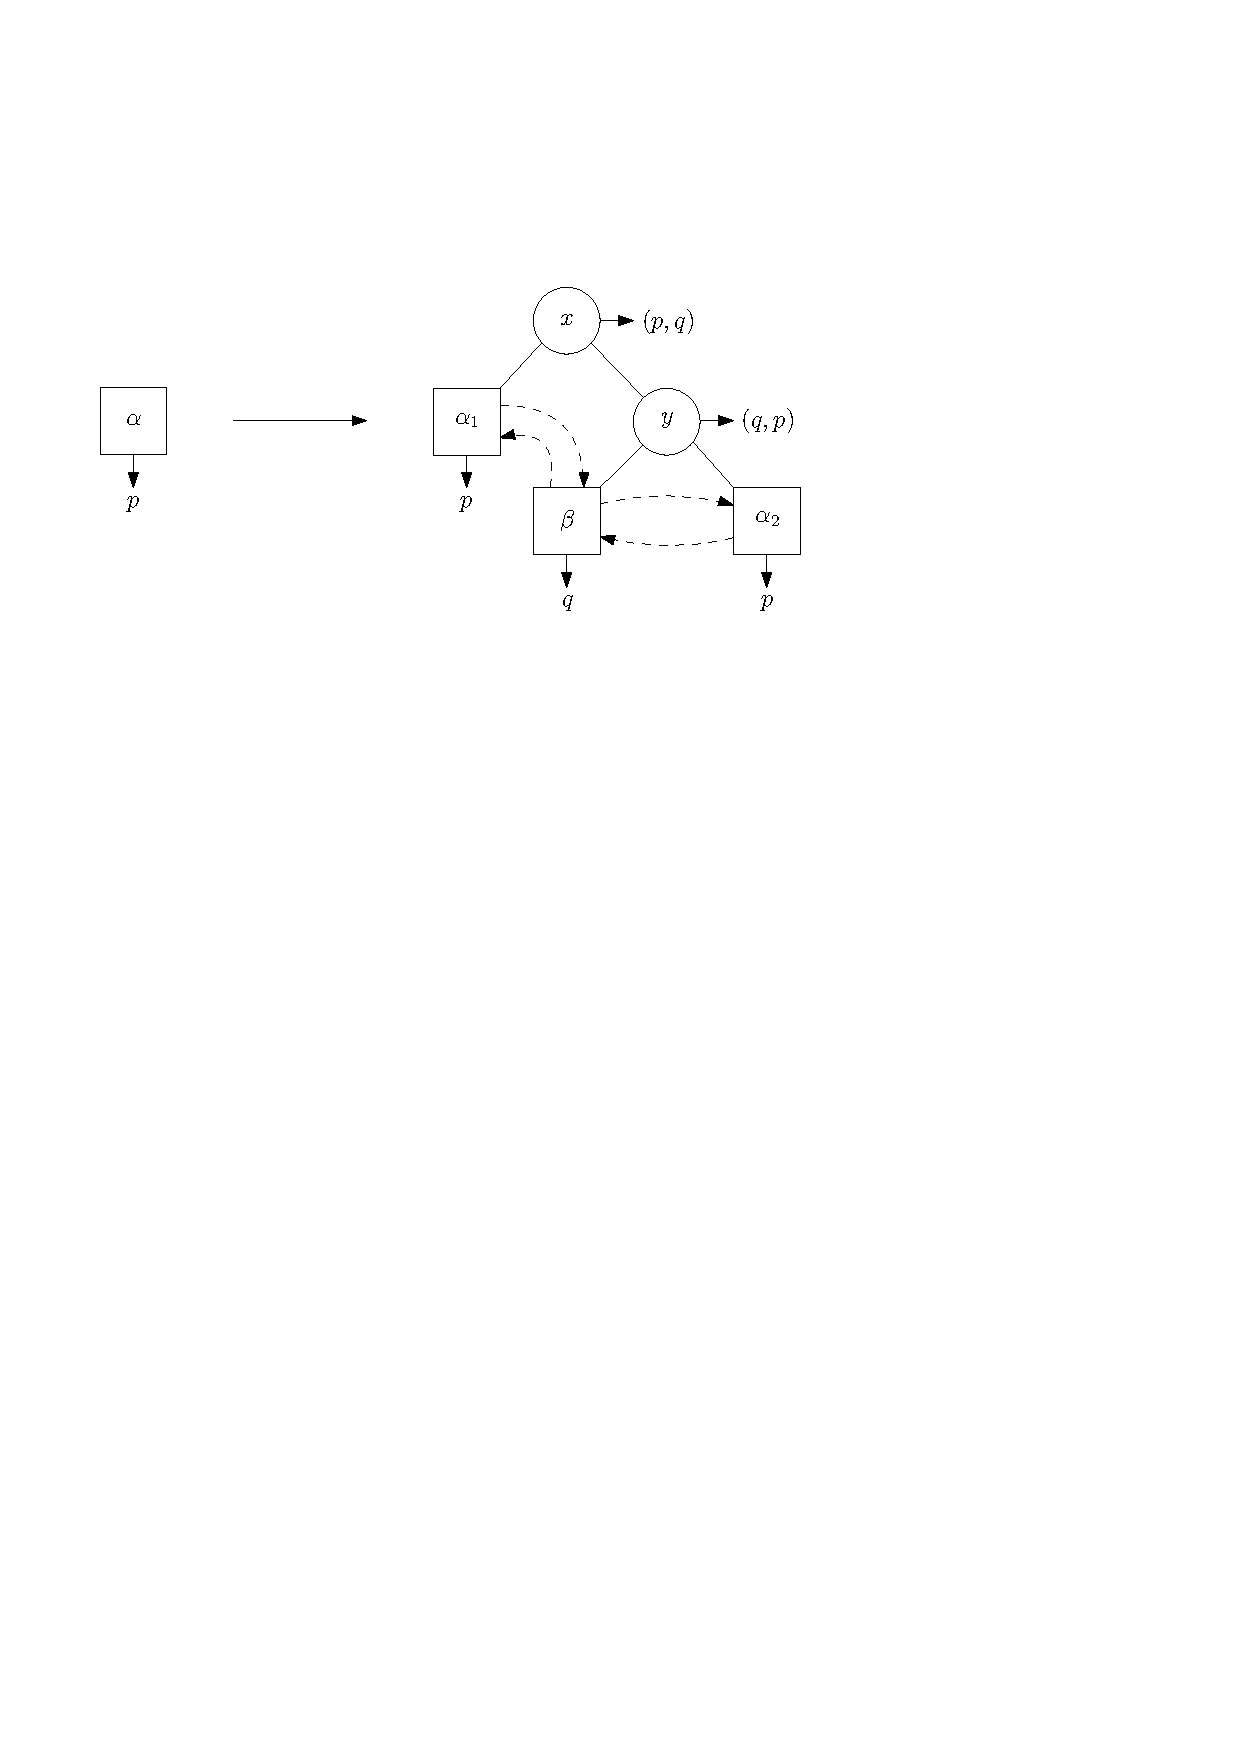
\includegraphics[scale=0.75]{images/tree_insert}
\]
The leaf $\alpha$ gets replaced by the tree on the right. The dashed arrows represent the pointers for our doubly-linked lists of arcs, and not depicted but also necessary is that we need to connect $\alpha_1$ to $\alpha$\textsf{.leftArc} and connect $\alpha_2$ to $\alpha$\textsf{.rightArc} by setting the appropriate pointers.

\todo{Describe how we delete from the tree at a circle event}
\[
    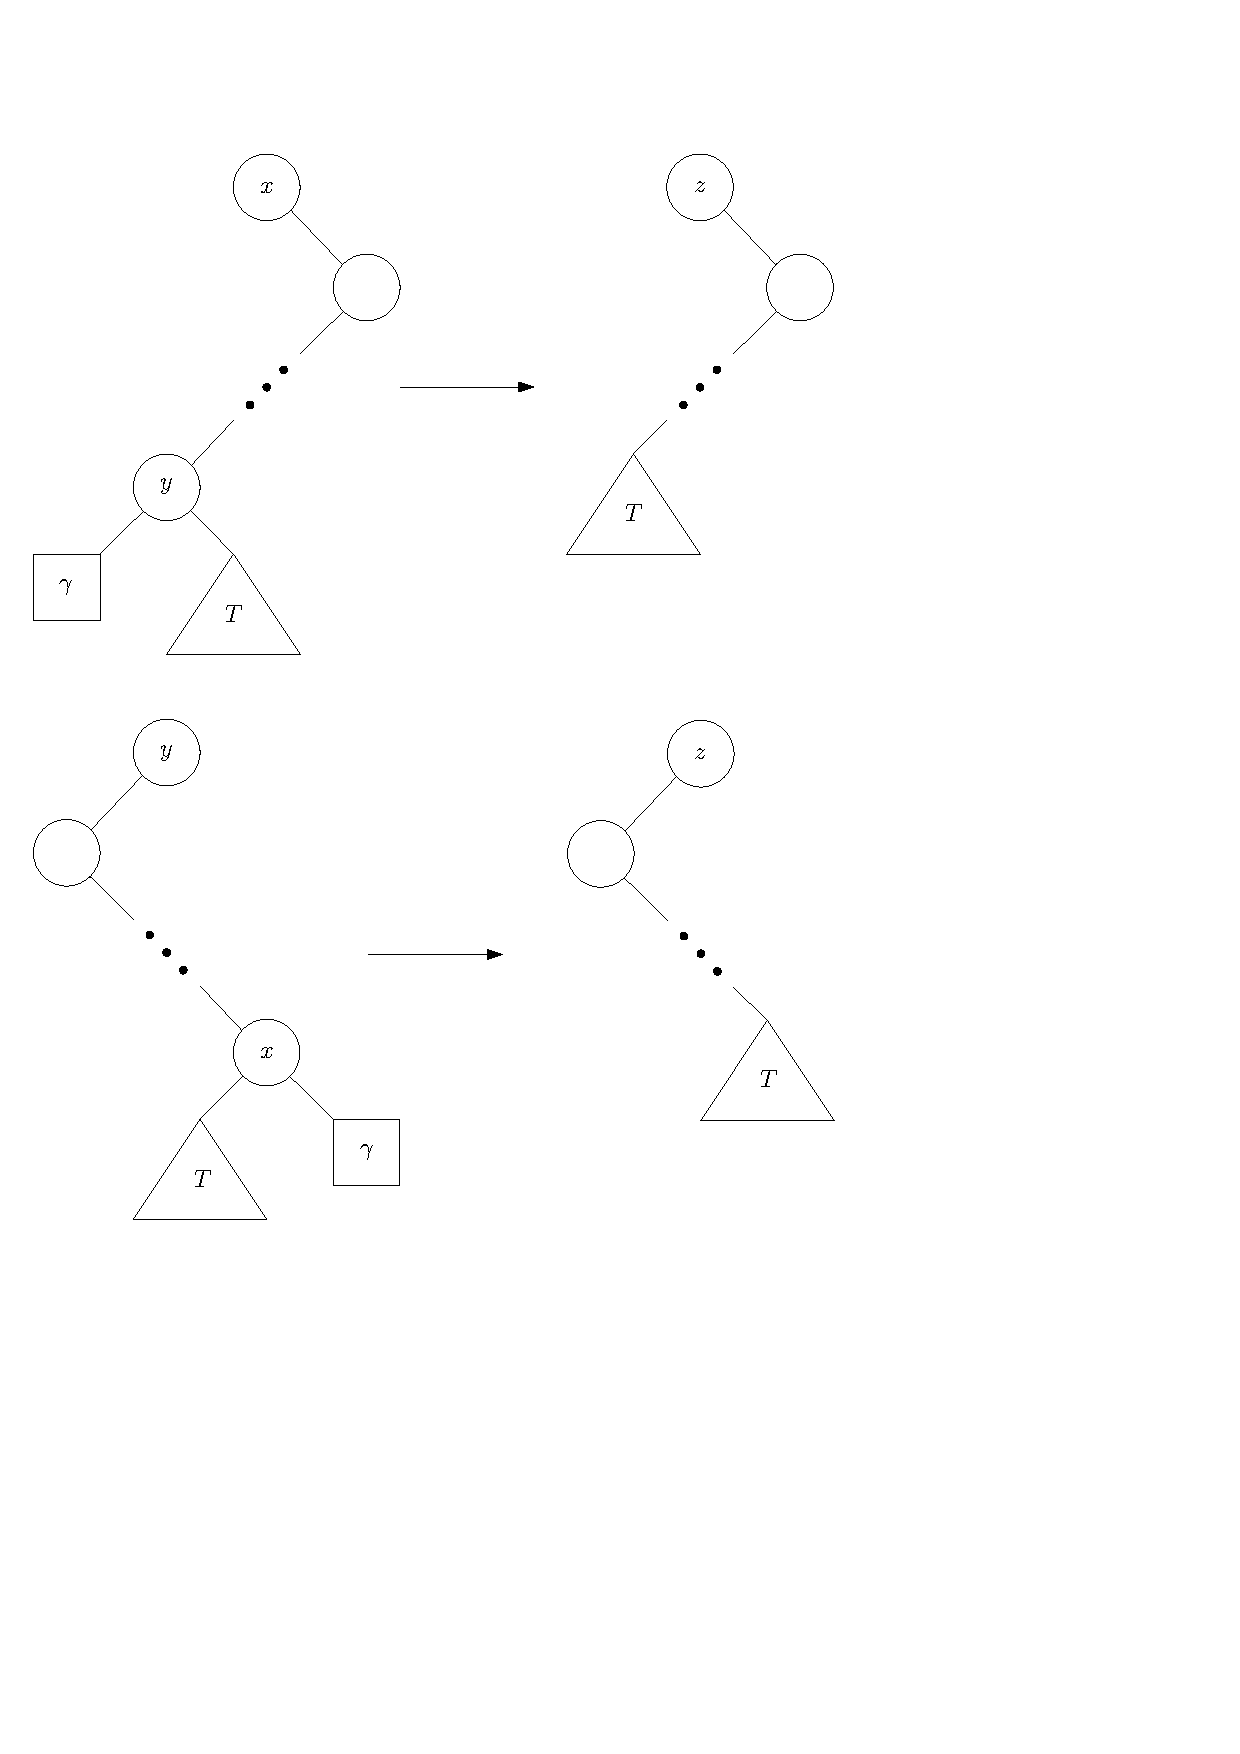
\includegraphics[scale=0.75]{images/tree_remove}
\]

\section{Doubly-connected edge list}

\todo{Describe how we modify the DCEL at a site event}

\todo{Describe how we modify the DCEL at a circle event}

\todo{Describe how we intersect the DCEL with a bounding box when we have been through the event queue}

\newpage
\section{Balancing the BST by using a treap}
There are multiple viable strategies for balancing a binary search tree. In this section we look at a particular strategy which utilizes randomness. We will introduce the treap data structure, which is a randomized self-balancing binary search tree. The presentation follows the paper \todo{Ref}, but only describes the things that we will need.

\begin{defn}[Treap]
Let $T$ be a tree where each node $x \in T$ has properties
\begin{itemize}
    \item $x\textsf{.left}$ is the left subtree of $x$,
    \item $x\textsf{.right}$ is the right subtree of $x$,
    \item $x\textsf{.key} \in \R$,
    \item $x\textsf{.priority} \in [0,1]$.
\end{itemize}
We say that $T$ is a \textit{treap} if
\begin{enumerate}[(i)]
    \item $T$ is a binary tree with respect to $\textsf{.key}$. That is, for every $x \in T$ we have
    \begin{align*}
        \forall y \in x\textsf{.left} &\colon y\textsf{.key} \leq x\textsf{.key}, \\
        \forall y \in x\textsf{.right} &\colon y\textsf{.key} \geq x\textsf{.key}.
    \end{align*}
    \item $T$ is a max-heap with respect to $\textsf{.priority}$, that is for each $x, y \in T$:
    \begin{align*}
        x \text{ is the parent of } y \implies x\textsf{.priority} \geq y\textsf{.priority}.
    \end{align*}
\end{enumerate}
\end{defn}

\begin{defn}[Left and right rotations]
Given a tree $T$ and two nodes $x, y \in T$ with subtrees $A, B, C$ the operations \textit{rotate left} and \textit{rotate right} are given as follows:
\[
    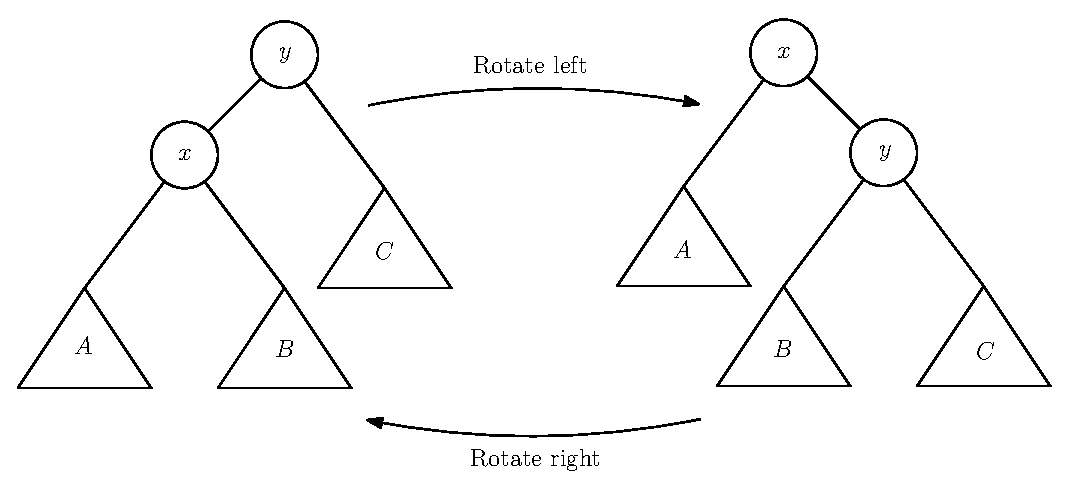
\includegraphics[width=\textwidth]{images/rotate}
\]
\end{defn}

From the diagram it is immediate that rotations preserve the binary tree property, but if $T$ has a $\textsf{.priority}$ property then the order on $x\textsf{.priority}$ and $y\textsf{.priority}$ is reversed. Given a binary tree $T$ with priorities we may then make sure it also has the max-heap property by making a finite sequence of left and right rotations, and thus we may turn it into a treap.

The basic operations on a treap are as follows:
\begin{itemize}
    \item $\textsc{Search}(x)$: This is the same as for a binary tree.
    \item $\textsc{Insert}(x)$: At first the insertion is identical to that of a binary tree: first we search for a spot to insert the new element, such that it stays a binary tree after insertion. Once inserted however, it may be the case that the max-heap property is violated. To remedy this, we may rotate $x$ up in the tree until the max-heap property is reestablished, or until we reach the root.
    \item $\textsc{Delete}(x)$: The strategy is to rotate $x$ down until it becomes a leaf in a manner which preserves the property that every subtree is a treap, and then we remove the leaf. This is done as follows: when rotating down we have a choice of rotating $x$ with the root $y$ of the left subtree $A$, or the root $z$ of the right subtree $B$. We choose to rotate $x$ and $y$ if $y\textsf{.priority} > z\textsf{.priority}$, otherwise we rotate $x$ and $z$, and then it follows by recursion that the treap property eventually is preserved in the entire tree once $x$ is a leaf, and then we clip away $x$.
\end{itemize}

\begin{defn}[Randomized search tree]
We define a \textit{randomized search tree} to be a treap $T$ where the priorities are independent, identically distributed continuous random variables.
\end{defn}

The main result we will work towards in this section is the following:

\begin{thm} \label{thm:treapmainthm}
A randomized search tree storing $n$ items has the expected performance characteristics listed in the table below:
\begin{table}[h!]
\centering
\begin{tabular}{ll}
\textbf{Performance measure}   & \textbf{Bound on expectation} \\ \hline
Search                         & $\mathcal{O}(\log n)$         \\
Insertion                      & $\mathcal{O}(\log n)$         \\
Deletion                       & $\mathcal{O}(\log n)$         \\
Number of rotations per update & $\leq 2$                      \\ \hline
\end{tabular}
\end{table}
\end{thm}
To prove this we will introduce some random variables and then we will work towards proving upper bounds for their expectations. The first random variables we introduce are:
\begin{itemize}
    \item $D(x)$: the number of nodes on the path from $x$ to the root.
    \item $SL(x)$ and $SR(x)$: the length of the right spine of the left subtree of $x$ and the length of the right spine of the right subtree of $x$. By length of the left spine of a tree we mean the number of nodes we pass if we keep following the left pointer from the root, and similarly for the right spine.
\end{itemize}
Throughout this section we will deal with a treap $T$ with nodes $x_1, x_2, \ldots, x_n$ where node $x_i$ has associated key $k_i$ and priority $p_i$, and $k_1 < k_2 < \cdots < k_n$. We now introduce the following indicator random variables:
\begin{align*}
    A_{i,j} &= \begin{cases}
        1 & \text{if } x_i \text{ is an ancestor of } x_j \text{ in } T, \\
        0 & \text{otherwise.}
    \end{cases} \\
    C_{i;\ell,m} &= \begin{cases}
        1 & \text{if } x_i \text{ is a common ancestor of } x_{\ell} \text{ and } x_{m} \text{ in } T, \\
        0 & \text{otherwise.}
    \end{cases}
\end{align*}
Note that we consider each node an ancestor of itself. We then have:
\begin{thm}
    Let $1 \leq \ell \leq n$. Then
    \begin{enumerate}[(i)]
        \item $D(x_{\ell}) = \sum_{i=1}^{n} A_{i,\ell}$.
        \item $SL(x_{\ell}) = \sum_{i=1}^{\ell-1} (A_{i,\ell-1} - C_{i;\ell-1,\ell})$.
        \item $SR(x_{\ell}) = \sum_{i=\ell+1}^{n} (A_{i,\ell+1} - C_{i;\ell,\ell+1})$.
    \end{enumerate}
\end{thm}
\begin{proof}
(i): Nodes on the path from $x_{\ell}$ to the root are exactly the nodes which $x_{\ell}$ has as ancestors.

(ii): First we assume that $x_{\ell}$ has a left subtree $L$. This has the nodes $x_i$ with $i < \ell$. The lowest node on the right spine of $L$ is $x_{\ell-1}$. This means that every node on the right spine of $L$ is an ancestor of $x_{\ell-1}$. Nodes in $L$ outside the right spine are not ancestors of $x_{\ell-1}$. Since none of the nodes in $L$ are ancestors of $x_{\ell}$ we have that $C_{i;\ell-1,\ell} = 0$ for all $i < \ell$, and hence the formula holds.

Now assume that $x_{\ell}$ has no left subtree. If $\ell = 1$ then the sum correctly evaluates to 0. If $\ell > 1$ then it must be the case that $x_{\ell-1}$ is an ancestor of $x_{\ell}$, and then every ancestor of $x_{\ell-1}$ is a common ancestor of $x_{\ell-1}$ and $x_{\ell}$, so the formula again correctly evaluates to 0.

(iii): This argument is symmetrical to the one for (ii).
\end{proof}

If we let $a_{i,j} = \mathbb{E}[A_{i,j}]$ and $c_{i;\ell,m} = \mathbb{E}[C_{i;\ell,m}]$ then by linearity of expectation we get:
\begin{cor}
Let $1 \leq \ell \leq n$ and let $\ell < m$. Then
    \begin{enumerate}[(i)]
        \item $\mathbb{E}[D(x_{\ell})] = \sum_{i=1}^{n} a_{i,\ell}$.
        \item $\mathbb{E}[SL(x_{\ell})] = \sum_{i=1}^{\ell-1} (a_{i,\ell-1} - c_{i;\ell-1,\ell})$.
        \item $\mathbb{E}[SR(x_{\ell})] = \sum_{i=\ell+1}^{n} (a_{i,\ell+1} - c_{i;\ell,\ell+1})$.
    \end{enumerate}
\end{cor}

Our analysis has now been reduced to determining the expectations $a_{i,j}$ and $c_{i;\ell,m}$. Now, if $X$ is an indicator random variable, then
\[
    \mathbb{E}[X] = \textsf{Pr}(X = 1),
\]
so we get that
\[
    a_{i,j} = \textsf{Pr}(A_{i,j} = 1) = \textsf{Pr}(x_i \text{ is an ancestor of } x_j)
\]
and
\[
    c_{i;\ell,m} = \textsf{Pr}(C_{i;\ell,m} = 1) = \textsf{Pr}(x_i \text{ is a common ancestor of } x_{\ell} \text{ and } x_{m}).
\]
Determining these probabilities is made possible through the ancestor lemma:
\begin{lem}[Ancestor lemma]
Assuming that all priorities are distinct, then $x_i$ is an ancestor of $x_j$ in $T$ if and only if $p_i \geq p_h$ for all $h$ in between and including $i$ and $j$.
\end{lem}
\begin{proof}
Let $x_m$ be the item with the highest priority in $T$. Let
\[
    L = \makeset{x_{\nu}}{1 \leq \nu < m}
    \quad
    \text{and}
    \quad
    R = \makeset{x_{\mu}}{m < \mu \leq n}.
\]
Note that since $x_m$ is the node with the highest priority in $T$ it is actually the root, so we may consider $L$ and $R$ as the left and right subtrees of $x_m$. Note that $L$ and $R$ are treaps also.

For every $x_{\ell} \in L$ we have that $x_m$ is an ancestor of $x_{\ell}$ and $p_m \geq p_h$ for all $\ell \leq h \leq m$. Thus it follows that any pair with $x_m$ and $x_{\ell} \in L$ satisfy the ancestor characterization. Similarly every pair with $x_m$ and any node in $R$ satisfies the characterization. Now, note that a pair with $x_i \in L$ and $x_j \in R$ trivially satisfy the characterization, as they are not ancestor related.

We may then by recursion use the same argument on $L$ and $R$, and this way we end out showing that the characterization is true for all pairs in $T$.
\end{proof}

\begin{lem}[Common ancestor lemma]
Let $1 \leq \ell, m, i \leq n$ with $\ell < m$. Assuming that all priorities are distinct, then $x_i$ is a common ancestor of $x_{\ell}$ and $x_m$ in T if and only if
\begin{equation} \label{eq:commonacenstorproperty}
    p_i = \max\makeset{p_{\nu}}{\min\curly{i,\ell,m} \leq \nu \leq \max\curly{i,\ell,m}}.
\end{equation}
\end{lem}
\begin{proof}
Equation (\ref{eq:commonacenstorproperty}) is equivalent to the following cases:
\begin{itemize}
    \item $p_i = \max\makeset{p_{\nu}}{i \leq \nu \leq m}$ if $1 \leq i \leq \ell$.
    \item $p_i = \max\makeset{p_{\nu}}{\ell \leq \nu \leq m}$ if $\ell \leq i \leq m$.
    \item $p_i = \max\makeset{p_{\nu}}{\ell \leq \nu \leq i}$ if $m \leq i \leq n$.
\end{itemize}
The fact that the lemma is true for each of these cases is a direct consequence of the ancestor lemma.
\end{proof}

\begin{cor} \label{cor:propofancestor}
$a_{i,j} = \displaystyle \frac{1}{\abs{i - j} + 1}$.
\end{cor}
\begin{proof}
By the ancestor lemma $x_i$ is an ancestor of $x_j$ if and only if
\[
    p_i = \max\makeset{p_h}{\min\curly{i, j} \leq h \leq \max\curly{i, j}}.
\]
Since the $p_i$ are independent and identically distributed continuous random variables, this happens with probability
\[
    \frac{1}{\abs{\makeset{h \in \N}{\min\curly{i, j} \leq h \leq \max\curly{i, j}}}} = \frac{1}{\abs{i - j} + 1}.
\]
\end{proof}

\begin{cor}
$c_{i;\ell,m} = \displaystyle \frac{1}{\max\curly{i,\ell,m} - \min\curly{i,\ell,m} + 1}$.
\end{cor}
\begin{proof}
By the common ancestor lemma $x_i$ is a common ancestor of $x_{\ell}$ and $x_m$ if and only if
\[
    p_i = \max\makeset{p_{\nu}}{\min\curly{i,\ell,m} \leq \nu \leq \max\curly{i,\ell,m}}.
\]
Like in the proof of Lemma \ref{cor:propofancestor} we then use that the $p_i$ are i.i.d to conclude that the probability is the reciprocal of the cardinality of the set we are taking the maximum of, and this cardinality is $\max\curly{i,\ell,m} - \min\curly{i,\ell,m} + 1$.
\end{proof}

Now we are ready to find upper bounds on the expectations of the quantities we are interested in. In order to do this, we will need the harmonic numbers, which are are given by $H_n = \sum_{i=1}^n \frac{1}{i}$. Their crucial property is the inequalities
\[
    \ln n < H_n < 1 + \ln n
\]
for all $n > 1$. \todo{Find proof or reference.}

\begin{thm} \label{thm:treapbounds}
Let $1 \leq \ell \leq m$. In a randomized search tree with $n$ nodes the following expectations hold:
\begin{enumerate}[(i)]
    \item $\mathbb{E}[D(x_{\ell})] = H_{\ell} + H_{n+1-\ell} - 1 < 1 + 2 \cdot \ln n = \mathcal{O}(\log n)$.
    \item $\mathbb{E}[SL(x_{\ell})] = 1 - \displaystyle \frac{1}{\ell}$.
    \item $\mathbb{E}[SR(x_{\ell})] = 1 - \displaystyle \frac{1}{n + 1 - \ell}$.
\end{enumerate}
\end{thm}
\begin{proof}
For (i) we get
\begin{align*}
    \mathbb{E}[D(x_{\ell})] &= \sum_{i=1}^n a_{i,\ell} \\
    &= \sum_{i=1}^n \frac{1}{\abs{i - \ell} + 1} \\
    &= \sum_{i=1}^{\ell} \frac{1}{\ell - i + 1} + \sum_{i=\ell}^{n} \frac{1}{i - \ell + 1} - 1 \\
    &= \sum_{i=1}^{\ell} \frac{1}{i} + \sum_{i=1}^{n+1-\ell} \frac{1}{i} - 1 \quad \text{(Reverse left sum and swap index in right)} \\
    &= H_{\ell} + H_{n+1-\ell} - 1 \\
    &< (1 + \ln \ell) + (1 + \ln (n + 1 - \ell)) - 1 \\
    &\leq 1 + 2 \cdot \ln n.
\end{align*}
For (ii) we have
\begin{align*}
    \mathbb{E}[SL(x_{\ell})] &= \sum_{i=1}^{\ell - 1} \left(a_{i,\ell-1} - c_{i;\ell-1,\ell}\right) \\
    &= \sum_{i=1}^{\ell - 1} \left(\frac{1}{\abs{i - (\ell - 1)} + 1} - \frac{1}{\max\curly{i,\ell-1,\ell}-\min\curly{i,\ell-1,\ell}+1}\right) \\
    &= \sum_{i=1}^{\ell - 1} \left(\frac{1}{\ell - i} - \frac{1}{\ell - i + 1}\right) \\
    &= \frac{1}{\ell - (\ell - 1)} - \frac{1}{\ell} \quad \text{(The above is a telescoping sum)} \\
    &= 1 - \frac{1}{\ell}.
\end{align*}
For (iii) we note that the proof is basically the same as for (ii) so we omit it.
\end{proof}

By combining Lemma \ref{lem:treapoperationsbounds} and Lemma \ref{lem:treaprotationbound} below we obtain a proof of Theorem \ref{thm:treapmainthm}, which will complete our analysis of treaps:

\begin{lem} \label{lem:treapoperationsbounds}
The operations \textsc{Search}, \textsc{Insert} and \textsc{Delete} take expected $\mathcal{O}(\log n)$ time.
\end{lem}
\begin{proof}
Searching for the spot for an element $x$ takes expected
\[
    \mathbb{E}[D(\textsc{Pred}(x)) + D(\textsc{Succ}(x))] = \mathcal{O}(\log n)
\]
time, where $\textsc{Pred}(x)$ finds a predecessor for $x$, e.g. finding the element in $T$ with the largest key less than or equal to $x\textsf{.key}$, and $\textsc{Succ}(x)$ finds a successor for $x$, e.g. finding the element in $T$ with the smallest key greater than or equal to $x\textsf{.key}$.

For insertion we first need to perform a search, and then afterwards the number of times we rotate is at most the length of the path traversed during search. The bound thus follows from the bound for search.

Since a deletion is basically just the reversal of an insertion the bounds follow.
\end{proof}

\begin{lem} \label{lem:treaprotationbound}
Let $x_{\ell}$ be an element of a treap which is to be deleted, or an element which has just been inserted into a treap. Let $R(x_{\ell})$ be the number of rotations which were needed during the update of the treap. Then $\mathbb{E}[R(x_{\ell})] \leq 2$.
\end{lem}
\begin{proof}
First, we note that since in terms of rotations a deletion is an exact reversal of an insertion it suffices to analyze the number of rotations that occur during a deletion. First, we note that if a node $x$ is right-rotated down, then $SL(x)$ decreases by one, and if a node $x$ is left-rotated down, then $SR(x)$ decreases by one. Once $x$ has been rotated down such that it is a leaf $y$, we have $SL(y) = SR(y) = 0$. It follows by recursion that $R(x) = SL(x) + SR(x)$. Then linearity of expectation and Theorem \ref{thm:treapbounds} gives us that
\[
    \mathbb{E}[R(x_{\ell})] = \mathbb{E}[SL(x_{\ell})] + \mathbb{E}[SR(x_{\ell})] = 2 - \para{\frac{1}{\ell} + \frac{1}{n + 1 - \ell}} \leq 2.
\]
\end{proof}